\vspace{-2mm}
\section{\ouralg：程序感知智能体推理系统}
\label{sec:thunder_agent}

基于 \autoref{sec:motivation} 中的发现，我们提出 \ouralg，一个用于高吞吐量智能体推理的程序感知系统。我们在 \autoref{sec:program_definition} 中建模智能体程序，这是系统调度的主要抽象。\autoref{sec:utility_model} 形式化了指导系统设计的成本模型。在这些基础上，我们进一步介绍 KV 缓存调度策略（\autoref{sec:scheduling_policy}）和工具资源管理策略（\autoref{sec:tool_resource}）。

\begin{table}[ht]
\caption{\textbf{智能体程序符号摘要。} 每个程序实例由其身份、执行阶段、工具环境、资源占用以及 \ouralg 中的调度状态刻画。}
\vspace{-1.5em}
\label{tab:notations}
\begin{center}
\small
\renewcommand{\arraystretch}{1.1}
\begin{tabularx}{\columnwidth}{lX}
\toprule
\textbf{符号} & \textbf{描述} \\
\midrule
$P$ & 智能体程序实例 \\
$\mathit{ID}$ & 程序的唯一全局标识符 \\
$c$ & 上下文中的标记数量 \\
$\mathcal{T}$ & 程序所需的工具环境集 \\
$\mathcal{L}$ & 空间局部性的后端（GPU 节点）放置 \\
$\tau$ & 执行阶段：推理（\textbf{R}），执行（\textbf{A}） \\
$s$ & 调度状态： $\{\text{Active, Paused, Terminated}\}$ \\
\bottomrule
\end{tabularx}
\end{center}
\vspace{-8mm}
\end{table}

\begin{figure*}[!t]
    \centering
    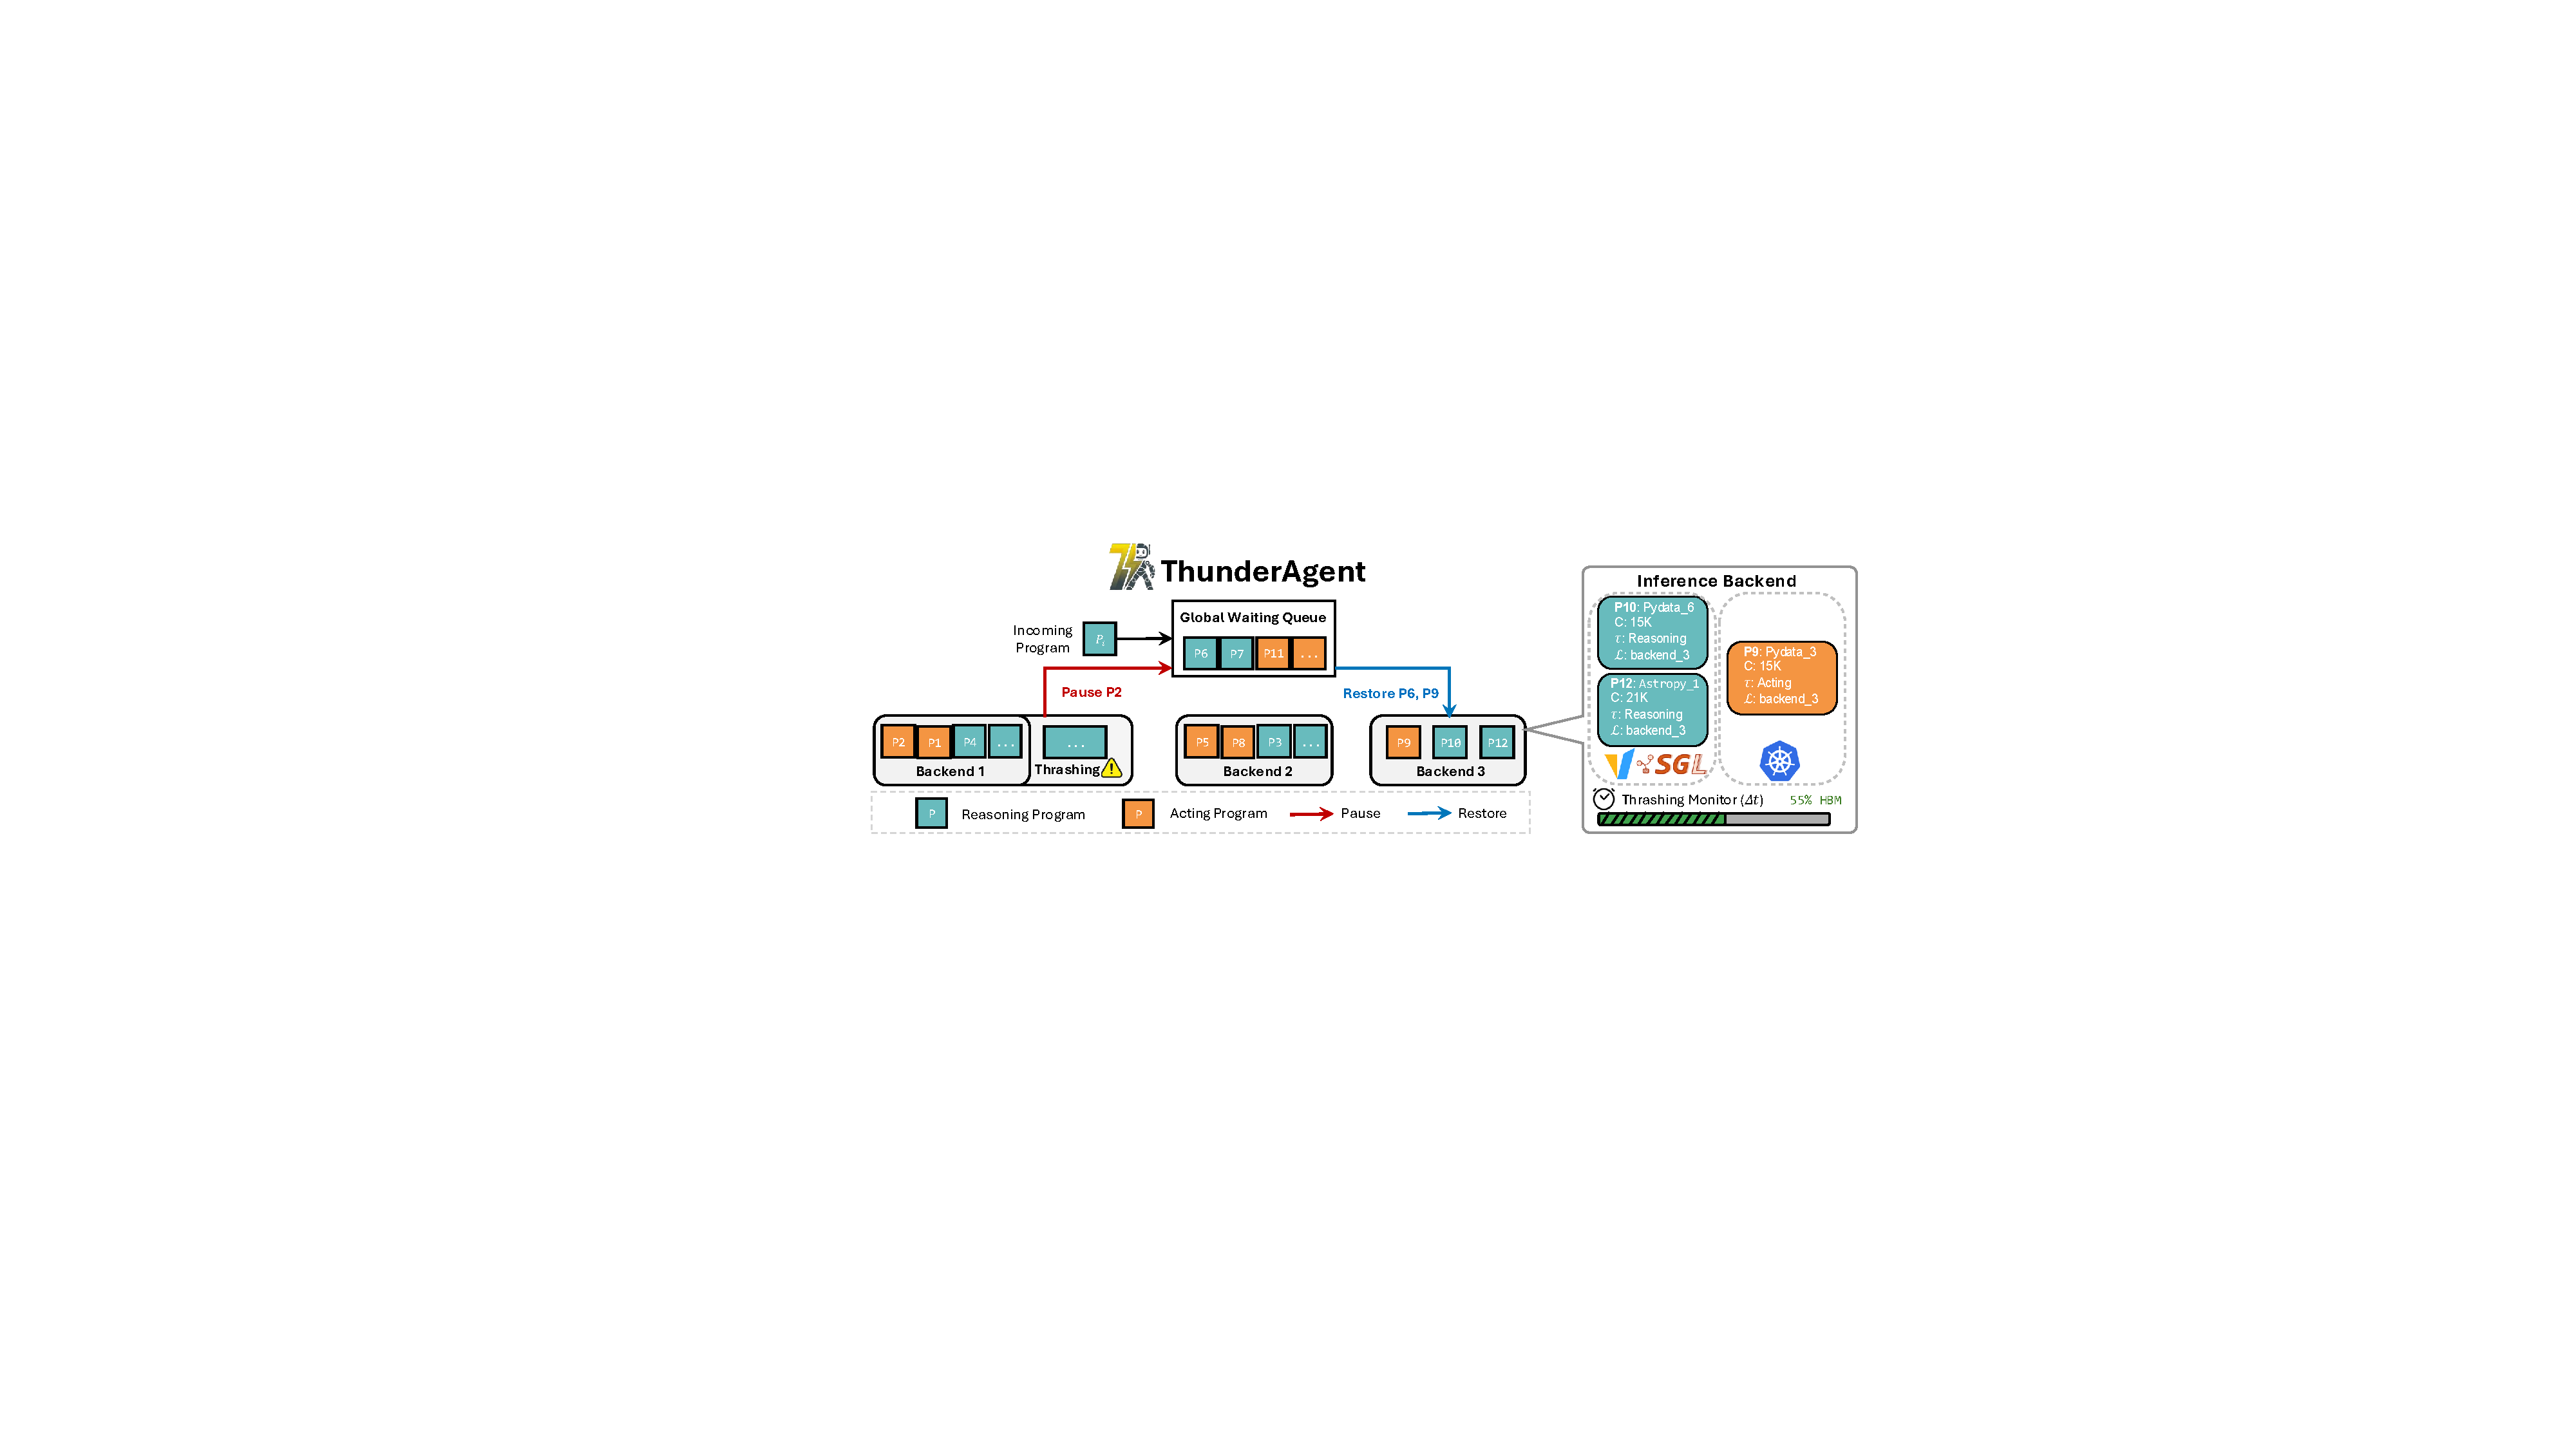
\includegraphics[width=1.0\columnwidth]{Figures/TR5.pdf}
    \caption{\textbf{\ouralg 概览。} \textmd{图中展示了调度状态与显存管理之间的转换。\ouralg 每隔 $\Delta t$ 定期查询各数据并行后端的状态。在这里，后端 \#1 触发抖动，而后端 \#3 利用不足。所有后端共享的全局等待队列会暂停并回收处于执行阶段的程序 \#2，同时释放推理阶段程序 \#6 和 \#9，以停止后端 \#1 中的 KV 缓存抖动，并降低后端 \#3 的显存不均衡。}
    % \junxiong{Should we say Reasoning Phase and Acting Phase instead of Reasoning Program and Acting Program. Because programs switch between reasoning and acting. Readers may get confused and think we don’t have different types of programs.} \junxiong{Need a few sentence to describe this. This figure shows how ThunderAgent manages agent programs across multiple inference backends to avoid KV-cache thrashing. Programs run in per-backend working pools and are labeled as Reasoning or Acting depends on their current execution status. When a backend becomes memory-pressured, ThunderAgent pauses a selected program (red arrow) and moves it into a global waiting queue, freeing HBM and stopping thrashing. When capacity becomes available elsewhere, backends resume programs from the global queue (blue arrow). We prioritize pausing the program in acting (P2) rather than pausing a program in reasoning (P4). }
    }
    \label{fig:arch}
    \vspace{-4mm}
\end{figure*}

% \begin{figure*}[t!]  % 使用 figure* 让图片跨越两栏
%     \centering
%     \begin{subfigure}{0.75\textwidth}
%         \centering
%         \includegraphics[width=0.99\textwidth]{Figures/TR3.pdf}  % 替换为你的图片路径
%         \caption{LMCache offload}
%         \label{fig:kv offload}
%     \end{subfigure}
%     \begin{subfigure}{0.20\textwidth}
%         \centering
%         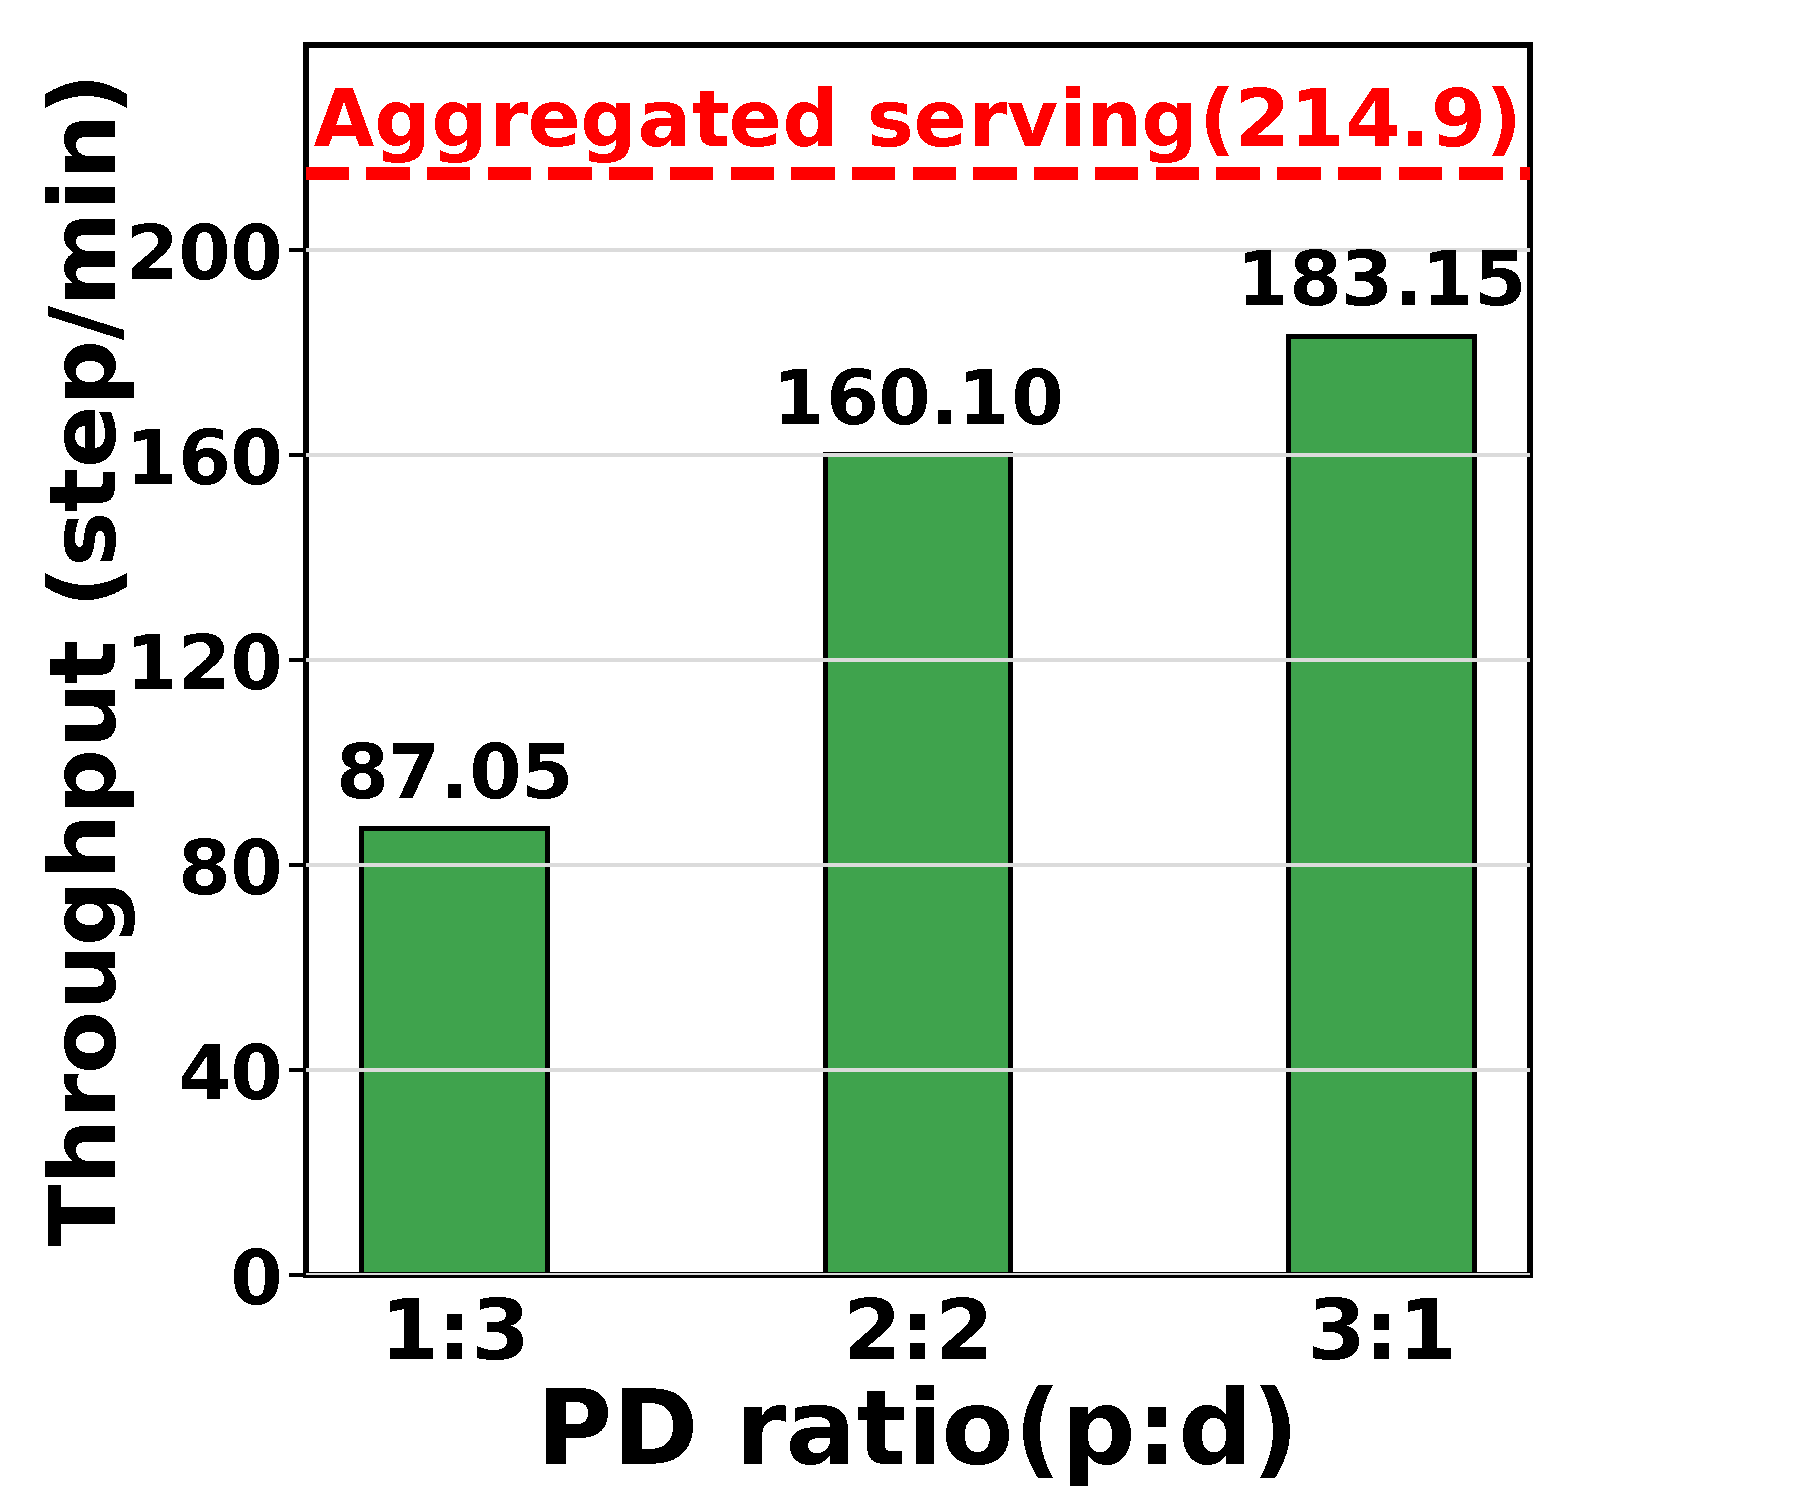
\includegraphics[width=0.99\textwidth]{Figures/throughput_vs_pd_ratio.pdf}  % 替换为你的图片路径
%         \caption{PD Disaggregation}
%         \label{fig:pd disaggregation}
%     \end{subfigure}
%     \vspace*{-0.2mm}
%     \caption{Ablation study of KV cache offload and prefill-decode disaggregation.}
%     \vspace{-4mm}
%     \label{fig:3}
% \end{figure*}
\subsection{程序抽象}
\label{sec:program_definition}
\textbf{智能体程序} 是一种基础抽象，用于封装智能体工作流的逻辑执行流和系统级依赖。形式化地，我们将智能体程序 $P$ 定义为如下元组：
\begin{align}
P = \langle \mathit{ID}, c, \mathcal{T}, \mathcal{L}, \tau, s \rangle,
\end{align}
% \vspace{-1mm}
\noindent 其中，$\mathit{ID}$ 表示唯一全局标识符。$c$ 表示上下文中的令牌数量，对应主动执行期间的 KV 缓存显存占用。$\mathcal{T}$ 跟踪程序使用的工具环境集合，使系统能在没有程序继续需要这些环境时进行垃圾回收。$\mathcal{L}$、$\tau$ 和 $s$ 分别表示节点放置、执行阶段和调度状态，从而支持程序级 KV 缓存抖动缓解和跨节点迁移。\autoref{fig:arch} 右侧给出了一个元数据示例。

\ouralg 通过对接 OpenAI 风格端点，直接封装现有 LLM 引擎和工具编排器。程序 ID 允许系统区分来自不同智能体工作流的请求。我们在附录~\ref{app:easy_intergrate} 中详细说明 \ouralg 与现有推理服务集成的简洁性。

\subsection{成本模型}
\label{sec:utility_model}

在多轮智能体推理过程中，只有用于主动预填充和解码的资源才有助于系统的有效吞吐量，而重新计算、已用容量和空闲缓存则构成资源浪费。我们将其包含在 GPU 资源消耗的成本模型中，该模型将有效成本与非生产性使用隔离开来。我们采用时空积（STP）~\citep{5388441} 作为我们的主要指标，定义为内存占用量随处理时间的积分。流程阶段的 STP 成本形式化为：
% \vspace{}
\begin{equation}
    \text{Cost}_{\text{x}} = \int_{0}^{t_{x}} M_x(t) \, dt,
\end{equation}
\noindent 在哪里 $t_x$ 是过程的持续时间 $x$ （例如，预填充）。由于内存使用 $M_x(t)$ 可以通过 LLM 中使用的 KV 缓存令牌计数直接量化，我们将成本模型定义为令牌计数随时间的积分。

智能体推理的总成本包括五个不同的部分：解码、预填充、重新计算、未使用的容量和空闲缓存。我们明确区分工具执行结果的增量预填充和历史交互的重新计算，后者由于在整个上下文上重新计算被逐出的 KV 缓存而导致成本显著升高。形式上，这会产生以下成本分解：
\begin{equation}
    \text{Cost}_{\text{total}} \approx \text{Cost}_{\text{decode}} + \text{Cost}_{\text{prefill}} + \text{Cost}_{\text{recompute}} +
    \text{Cost}_{\text{unused}} + \text{Cost}_{\text{caching}}
    \label{eq:cost_decomp}
\end{equation}
\noindent 在这个分解中， $\text{Cost}_{\text{decode}}$ 和  $\text{Cost}_{\text{prefill}}$ 代表有助于推理吞吐量的有效工作。其余的项都是浪费的系统开销： $\text{Cost}_{\text{recompute}}$ 源于 KV 缓存抖动（\autoref{sec:kv cache management}); $\text{Cost}_{\text{unused}}$ 反映数据并行 (DP) 推理后端副本之间的显存不均衡（\autoref{sec:cross node imbalance}）；和 $\text{Cost}_{\text{caching}}$ 在外部工具执行期间保持内存的同时进行累加（\autoref{sec:Tool mismanagement}).

\subsection{调度策略}
\label{sec:scheduling_policy}
基于上面的成本模型，我们的调度策略的优化目标是最小化非生产性开销部分： $\text{Cost}_{\text{recompute}}$, $\text{Cost}_{\text{unused}}$， 和 $\text{Cost}_{\text{caching}}$，从而最大化吞吐量。

\subsubsection{通过程序感知等待队列减少重新计算和缓存成本}
\label{sec:4.3.1}
正如所确定的 \autoref{sec:kv cache management} 和 \autoref{fig:workload_profile}，KV 缓存抖动是吞吐量下降的主要瓶颈。为了解决这个限制，系统必须最小化 $\text{Cost}_{\text{recompute}}$ 通过明确控制活动程序的数量。 \ouralg 通过引入程序感知的等待队列来实现这一点。我们的系统利用这个队列来调度器执行，根据令牌长度确定哪些程序应该在 GPU 中执行，哪些程序应该被换出 $c$ 和执行阶段 $\tau$。在这里，我们使用两个原始操作来形式化调度器行为： \textbf{恢复} 和 \textbf{暂停}，如下。

\begin{itemize}[itemsep=0.0pt,topsep=0pt,leftmargin=*]
    \item \textbf{恢复。} 此操作允许程序进入活动执行状态。给定一个程序 $P = \langle \mathit{ID}, c, \mathcal{T}, \mathcal{L}, \tau, s \rangle$ 和 $s = \text{Paused}$ 和 $\mathcal{L} = \varnothing$,
  恢复$(P)$ 分配 $P$ 到后端 $\mathcal{L}'$ 具有可用容量和更新
  \begin{align}
  P \leftarrow \langle \mathit{ID}, c, \mathcal{T}, \mathcal{L}', \tau, \text{Active} \rangle,
  \end{align}
    \item \textbf{暂停。} 此操作将程序从活动执行中删除。
给定一个程序 $P = \langle \mathit{ID}, c, \mathcal{T}, \mathcal{L}, \tau, s \rangle$
和 $s = \text{Active}$,
暂停$(P)$ 解除绑定 $P$ 从其后端释放其 KV 缓存以进行抢占，并更新
\begin{align}
P \leftarrow \langle \mathit{ID}, c, \mathcal{T}, \varnothing, \tau, \text{Paused} \rangle .
\end{align}
\end{itemize}

\noindent 基于这两个操作，我们接下来介绍我们的调度策略，以最大限度地减少 KV 缓存抖动。

\paragraph{定期抖动检测。}  程序抽象为 \autoref{sec:program_definition} 为我们提供了智能体程序的KV 缓存大小。值得注意的是，这在请求级系统中不可用（如 \autoref{sec:motivation}）。我们定义 DP 后端的抖动条件 $\mathcal{L}$ 当程序内存需求超过总容量时：
\begin{equation}
    \text{C}_{\text{total}} < \sum_{p \in \mathcal{L}} c_p
\end{equation}
\noindent 在哪里 $\text{C}_{\text{total}}$ 表示后端KV 缓存池的固定token容量 $\mathcal{L}$。在解码过程中，上下文长度 $c_p$ 智能体工作流的数量快速增长，这可能会引发内存抖动 \emph{执行中期} 即使没有新来者。与仅在工作流到达时执行是否接纳工作流的检查的基线调度器（例如，Continuum）不同，我们实现了 \textbf{定期监测} 以固定时间间隔评估内存使用情况 $\Delta t$, \mbox{允许抢先检测并减轻上下文增长引起的显存压力。}

当 KV 缓存抖动即将发生时， \ouralg 调用 \textbf{暂停} 暂停活动程序和释放内存大小的操作 $\Delta C = \sum_{p \in \mathcal{L}} c_p - \lambda_{\max} \cdot \text{C}_{\text{total}}$ 直到总内存使用量低于限制 $\lambda_{\max} \cdot \text{C}_{\text{total}}$。相反，当后端有可用空间时，意味着
$\sum_{p \in \mathcal{L}} c_p < \lambda_{\min} \cdot C_{\text{total}}$, \ouralg 通过以下方式从等待队列中恢复暂停的程序 \textbf{恢复}，确保恢复的程序保持总内存低于 $\lambda_{\max} \cdot \text{C}_{\text{total}}$。这里， $\lambda_{\max}$ 和 $\lambda_{\min}$ 表示高水位线和低水位线
的内存使用情况，分别共同形成一个滞后窗口
稳定我们的日程安排。在实践中，我们将这两个值都设置为 1，因为跨程序的共享提示隐式保留了足够的内存缓冲区。

通过此程序级定期容量检查， \ouralg 可以通过在执行阶段为活动程序保留内存来保证不会出现 KV 缓存抖动。然而，代价是当程序进行长时间运行的工具执行时，执行程序占用的 GPU 显存处于空闲状态。为了平衡缓存与重新计算的成本，我们将时间衰减机制纳入抖动检查中，逐步降低执行程序令牌的有效权重。这允许调度器在显存压力上升时驱逐长时间空闲的缓存，而不是无限期地保留它们：
\begin{equation}
\label{eq:time_decay}
    \text{C}_{\text{total}} < \sum_{p \in \mathcal{L},\tau = \textbf{R}} c_p +\sum_{q \in \mathcal{L},\tau = \textbf{A}} c_q \times f(t_q)
\end{equation}
具体来说， $t_q$ 是程序的工具执行时间 $q$ 在当前步骤中。 $f(t)$ 是一个时间衰减函数，旨在平衡 $\text{Cost}_{\text{caching}}$ 和 $\text{Cost}_{\text{recompute}}$。通过随着时间的推移动态降低正在执行的程序的有效内存优先级， $f(t)$ 鼓励调度器驱逐保持空闲的缓存。
在 \autoref{app:ft_discussion}，我们证明当工具执行延迟满足无记忆属性（即剩余执行时间与经过的持续时间无关）时，最优衰减函数 $f(t)$ 采取指数衰减的形式。

\paragraph{最小化 $\text{Cost}_{\text{recompute}}$ 通过最短优先驱逐。}
有了上述驱逐和恢复条件，处理抖动的剩余问题是确定暂停活动程序的哪个子集，以使重新计算成本最小化。在本段中，我们证明了驱逐具有最小 KV 缓存大小的程序会产生最佳解决方案，详细证明参见 \autoref{app:prefill_stpcost}.

\begin{lemma}[Quadratic Recomputation Cost]
\label{lem:recompute_quadratic}
给定一个程序 $P_i$ 与上下文长度 $c_i$，重新填充其 KV 缓存所产生的重新计算成本与 $c_i$， IE。，
\begin{equation}
    \text{Cost}_{\text{recompute}} = \int_{0}^{t_{\mathrm{recompute}}} c_i(t) \, dt \propto c_i^2.
\end{equation}
\end{lemma}

\begin{definition}[Eviction Optimization Problem]
\label{def:eviction_problem}
基于引理~\ref{lem:recompute_quadratic}，给定所需的内存释放 $\Delta C$，调度器的目标是
选择一个子集 $S$ 的程序驱逐，以便释放
容量满足约束，同时最小化总容量
重新计算成本。该优化问题表述如下：
\begin{equation}
\min_{S} \sum_{i \in S} c_i^2
\quad \text{s.t.} \quad
\sum_{i \in S} c_i \ge \Delta C.
\end{equation}
\end{definition}

目标通过选择较小的 $c_i$ 得到严格最小化。因此，\ouralg 的策略是贪婪地暂停并驱逐具有 \textbf{最短上下文长度} 的程序。形式化证明见附录~\ref{app:_minimized_STP_cost}。基于这些分析，我们在调度器中使用以下分数来恢复和暂停程序：
\begin{equation}
    S_{\mathrm{restore}}(P) = \frac{1}{c_P} + \mathbb{I}(\tau = \textbf{R})
\end{equation}
\begin{equation}
    S_{\mathrm{pause}}(P) = \frac{1}{c_P} + \mathbb{I}(\tau = \textbf{A})
    \end{equation}
\noindent 其中指标函数 $\mathbb{I}(\cdot)$ 强制执行程序执行状态的严格优先级（$\tau$）超过上下文长度。两种机制都遵循 \textbf{最短优先} 最小化重新计算成本的策略。然而，状态指示器 $\mathbb{I}$ 确保调度器优先考虑暂停智能体程序，从而最大限度地减少 $\text{Cost}_{\text{caching}}$ 通过回收缓存内存，同时优先考虑恢复推理程序以最大化 $\text{Cost}_{\text{decode}} + \text{Cost}_{\text{prefill}}$.

\subsubsection{通过全局程序感知等待队列减少显存不均衡}
\autoref{sec:kv cache management} 和 \autoref{fig:dp unbalance} 强调节点之间的显存不均衡会带来显著的影响 $\text{Cost}_{\text{unused}}$，尽管其他节点有足够的GPU 显存容量，但仍会导致不必要的程序暂停。为此， \ouralg 将所有后端副本的等待队列统一为一个 \textbf{全局程序感知等待队列}。

这个设计的关键动机是 $\text{Cost}_{\text{unused}}$ 仅出现
当暂停的程序仍在等待队列中，而某些副本
有闲置内存。而且，一旦程序暂停，它的KV 缓存就会被
假设被驱逐，使其重新计算成本与节点无关。这使我们能够在不牺牲 KV 缓存局部性的情况下改善跨节点内存平衡。恢复策略与负载平衡相一致，而不是严格的 KV 感知路由，使暂停的程序能够调度到任何
具有可用GPU 显存容量的副本。因此，全局队列限制了未使用的成本，使得 $\text{C}_{\text{unused}} < c_{\mathrm{min}} \cdot \Delta t$\footnote{自从 $\Delta t$ 比程序的生命周期小得多，我们忽略单个时间间隔内终止程序的影响。} 对于周期内的每个节点 $\Delta t$， 在哪里 $c_{\mathrm{min}}$ 表示暂停程序中的最小令牌长度。调度策略和全局等待队列概述 \ouralg 提出于 \autoref{fig:arch}.

\subsection{工具资源管理}
\label{sec:tool_resource}
下一个， \ouralg 减轻资源泄漏和环境设置开销，详见 \autoref{sec:Tool mismanagement}.
% , using the program-aware abstraction.
\paragraph{基于钩子的垃圾收集。} 我们实现了生命周期钩子，将工具资源的持久性与智能体程序的调度状态严格耦合起来 $s$。当一个程序是 \textit{终止}，收集器立即触发拆卸序列，系统地回收沙箱、网络套接字和计算槽。活动磁盘使用情况 \autoref{fig:disk mem} 展示了我们的资源管理策略有效地防止了过多资源的积累，随着时间的推移保持了近乎恒定的磁盘空间占用。


\paragraph{异步环境准备。} 初始化工具执行环境所涉及的延迟
 （例如，启动 Docker 容器并安装依赖项）可能是瓶颈。为了解决这个问题， \ouralg 监控全局等待队列；当高优先级程序（高 $S_\text{restore}$）接近恢复阈值时，系统会在分配 GPU 显存之前异步恢复其执行环境。这项技术有效地 \textbf{隐藏初始化开销}，显著减少工具调用繁重工作负载（例如编码智能体和科学智能体）的端到端延迟，如 \autoref{fig:env prepare}.
